\documentclass[tikz]{standalone}

\usetikzlibrary{calc,angles,positioning}

\begin{document}
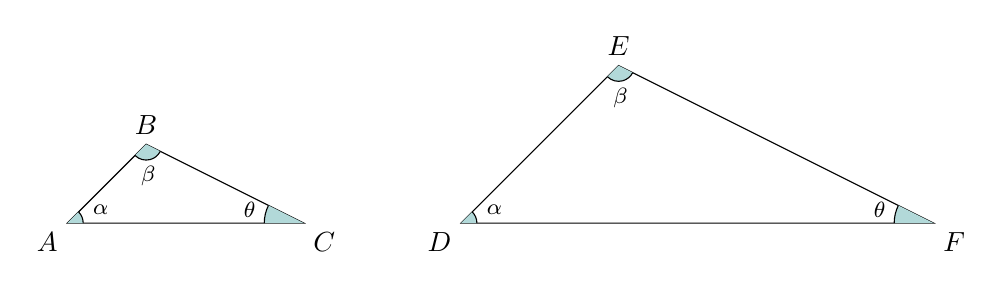
\begin{tikzpicture}[
        my angle/.style = {
            draw,
            fill=teal!30,
            angle radius=2mm,
            angle eccentricity=1.1,
            font=\footnotesize}
    ]
    \coordinate (A) at (0,0);
    \coordinate (B) at (1,1);
    \coordinate (C) at (3,0);
    \draw (A) -- (B) -- (C) -- cycle;
    \path pic [my angle, anchor = -160, pic text=$\alpha$] {angle = C--A--B};
    \path pic [my angle, angle eccentricity = 0.8, anchor = 90, pic text = $\beta$] {angle = A--B--C};
    \path pic [
        my angle,
        angle radius = 0.5cm,
        angle eccentricity = 1,
        anchor = -15,
        pic text = $\theta$
    ] {angle = B--C--A};
    \node[below left] at (A) {$A$};
    \node[above] at (B) {$B$};
    \node[below right] at (C) {$C$};

    \coordinate (D) at (5,0);
    \coordinate (E) at (7,2);
    \coordinate (F) at (11,0);
    \draw (D) -- (E) -- (F) -- cycle;
    \path pic [my angle, anchor = -160, pic text=$\alpha$] {angle = F--D--E};
    \path pic [my angle, angle eccentricity = 0.8, anchor = 90, pic text = $\beta$] {angle = D--E--F};
    \path pic [
        my angle,
        angle radius = 0.5cm,
        angle eccentricity = 1,
        anchor = -15,
        pic text = $\theta$] {angle = E--F--D};
    \node[below left] at (D) {$D$};
    \node[above] at (E) {$E$};
    \node[below right] at (F) {$F$};
\end{tikzpicture}
\end{document}
